% Options for packages loaded elsewhere
\PassOptionsToPackage{unicode}{hyperref}
\PassOptionsToPackage{hyphens}{url}
\PassOptionsToPackage{dvipsnames,svgnames,x11names}{xcolor}
%
\documentclass[
  a4paper,
  landscape]{scrreprt}

\usepackage{amsmath,amssymb}
\usepackage{iftex}
\ifPDFTeX
  \usepackage[T1]{fontenc}
  \usepackage[utf8]{inputenc}
  \usepackage{textcomp} % provide euro and other symbols
\else % if luatex or xetex
  \usepackage{unicode-math}
  \defaultfontfeatures{Scale=MatchLowercase}
  \defaultfontfeatures[\rmfamily]{Ligatures=TeX,Scale=1}
\fi
\usepackage{lmodern}
\ifPDFTeX\else  
    % xetex/luatex font selection
    \setmainfont[]{Times New Roman}
\fi
% Use upquote if available, for straight quotes in verbatim environments
\IfFileExists{upquote.sty}{\usepackage{upquote}}{}
\IfFileExists{microtype.sty}{% use microtype if available
  \usepackage[]{microtype}
  \UseMicrotypeSet[protrusion]{basicmath} % disable protrusion for tt fonts
}{}
\usepackage{xcolor}
\usepackage[inner=3cm,outer=2.54cm,top=2.54cm,bottom=2.54cm,headsep=10pt,headheight=100pt,footskip=33pt,ignorehead,ignorefoot,heightrounded]{geometry}
\setlength{\emergencystretch}{3em} % prevent overfull lines
\setcounter{secnumdepth}{-\maxdimen} % remove section numbering
% Make \paragraph and \subparagraph free-standing
\makeatletter
\ifx\paragraph\undefined\else
  \let\oldparagraph\paragraph
  \renewcommand{\paragraph}{
    \@ifstar
      \xxxParagraphStar
      \xxxParagraphNoStar
  }
  \newcommand{\xxxParagraphStar}[1]{\oldparagraph*{#1}\mbox{}}
  \newcommand{\xxxParagraphNoStar}[1]{\oldparagraph{#1}\mbox{}}
\fi
\ifx\subparagraph\undefined\else
  \let\oldsubparagraph\subparagraph
  \renewcommand{\subparagraph}{
    \@ifstar
      \xxxSubParagraphStar
      \xxxSubParagraphNoStar
  }
  \newcommand{\xxxSubParagraphStar}[1]{\oldsubparagraph*{#1}\mbox{}}
  \newcommand{\xxxSubParagraphNoStar}[1]{\oldsubparagraph{#1}\mbox{}}
\fi
\makeatother


\providecommand{\tightlist}{%
  \setlength{\itemsep}{0pt}\setlength{\parskip}{0pt}}\usepackage{longtable,booktabs,array}
\usepackage{calc} % for calculating minipage widths
% Correct order of tables after \paragraph or \subparagraph
\usepackage{etoolbox}
\makeatletter
\patchcmd\longtable{\par}{\if@noskipsec\mbox{}\fi\par}{}{}
\makeatother
% Allow footnotes in longtable head/foot
\IfFileExists{footnotehyper.sty}{\usepackage{footnotehyper}}{\usepackage{footnote}}
\makesavenoteenv{longtable}
\usepackage{graphicx}
\makeatletter
\def\maxwidth{\ifdim\Gin@nat@width>\linewidth\linewidth\else\Gin@nat@width\fi}
\def\maxheight{\ifdim\Gin@nat@height>\textheight\textheight\else\Gin@nat@height\fi}
\makeatother
% Scale images if necessary, so that they will not overflow the page
% margins by default, and it is still possible to overwrite the defaults
% using explicit options in \includegraphics[width, height, ...]{}
\setkeys{Gin}{width=\maxwidth,height=\maxheight,keepaspectratio}
% Set default figure placement to htbp
\makeatletter
\def\fps@figure{htbp}
\makeatother
% definitions for citeproc citations
\NewDocumentCommand\citeproctext{}{}
\NewDocumentCommand\citeproc{mm}{%
  \begingroup\def\citeproctext{#2}\cite{#1}\endgroup}
\makeatletter
 % allow citations to break across lines
 \let\@cite@ofmt\@firstofone
 % avoid brackets around text for \cite:
 \def\@biblabel#1{}
 \def\@cite#1#2{{#1\if@tempswa , #2\fi}}
\makeatother
\newlength{\cslhangindent}
\setlength{\cslhangindent}{1.5em}
\newlength{\csllabelwidth}
\setlength{\csllabelwidth}{3em}
\newenvironment{CSLReferences}[2] % #1 hanging-indent, #2 entry-spacing
 {\begin{list}{}{%
  \setlength{\itemindent}{0pt}
  \setlength{\leftmargin}{0pt}
  \setlength{\parsep}{0pt}
  % turn on hanging indent if param 1 is 1
  \ifodd #1
   \setlength{\leftmargin}{\cslhangindent}
   \setlength{\itemindent}{-1\cslhangindent}
  \fi
  % set entry spacing
  \setlength{\itemsep}{#2\baselineskip}}}
 {\end{list}}
\usepackage{calc}
\newcommand{\CSLBlock}[1]{\hfill\break\parbox[t]{\linewidth}{\strut\ignorespaces#1\strut}}
\newcommand{\CSLLeftMargin}[1]{\parbox[t]{\csllabelwidth}{\strut#1\strut}}
\newcommand{\CSLRightInline}[1]{\parbox[t]{\linewidth - \csllabelwidth}{\strut#1\strut}}
\newcommand{\CSLIndent}[1]{\hspace{\cslhangindent}#1}

\usepackage{scrlayer-scrpage}
\usepackage{graphicx}

\pagestyle{scrheadings}

\rofoot{Community-Health-Assessment}
% \rohead{
\includegraphics[width=4cm, height=4cm]{pages/Attachments/logo_PNM.png}}

% Ensure the header is on every page, including the first page of each chapter
\renewcommand*{\chapterpagestyle}{scrheadings}

% Adjust chapter title spacing
\makeatletter
\renewcommand*{\chapterheadstartvskip}{\vspace*{-0.5cm}} % Adjust this value to control the space before the chapter title
\renewcommand*{\chapterheadendvskip}{\vspace*{0.5cm}}  % Adjust this value to control the space after the chapter title
\makeatother
\makeatletter
\@ifpackageloaded{bookmark}{}{\usepackage{bookmark}}
\makeatother
\makeatletter
\@ifpackageloaded{caption}{}{\usepackage{caption}}
\AtBeginDocument{%
\ifdefined\contentsname
  \renewcommand*\contentsname{Table of contents}
\else
  \newcommand\contentsname{Table of contents}
\fi
\ifdefined\listfigurename
  \renewcommand*\listfigurename{List of Figures}
\else
  \newcommand\listfigurename{List of Figures}
\fi
\ifdefined\listtablename
  \renewcommand*\listtablename{List of Tables}
\else
  \newcommand\listtablename{List of Tables}
\fi
\ifdefined\figurename
  \renewcommand*\figurename{Figure}
\else
  \newcommand\figurename{Figure}
\fi
\ifdefined\tablename
  \renewcommand*\tablename{Table}
\else
  \newcommand\tablename{Table}
\fi
}
\@ifpackageloaded{float}{}{\usepackage{float}}
\floatstyle{ruled}
\@ifundefined{c@chapter}{\newfloat{codelisting}{h}{lop}}{\newfloat{codelisting}{h}{lop}[chapter]}
\floatname{codelisting}{Listing}
\newcommand*\listoflistings{\listof{codelisting}{List of Listings}}
\makeatother
\makeatletter
\makeatother
\makeatletter
\@ifpackageloaded{caption}{}{\usepackage{caption}}
\@ifpackageloaded{subcaption}{}{\usepackage{subcaption}}
\makeatother

\ifLuaTeX
  \usepackage{selnolig}  % disable illegal ligatures
\fi
\usepackage{bookmark}

\IfFileExists{xurl.sty}{\usepackage{xurl}}{} % add URL line breaks if available
\urlstyle{same} % disable monospaced font for URLs
\hypersetup{
  pdftitle={Community Health Needs Assessment},
  colorlinks=true,
  linkcolor={blue},
  filecolor={Maroon},
  citecolor={Blue},
  urlcolor={Blue},
  pdfcreator={LaTeX via pandoc}}


\title{Community Health Needs Assessment}
\usepackage{etoolbox}
\makeatletter
\providecommand{\subtitle}[1]{% add subtitle to \maketitle
  \apptocmd{\@title}{\par {\large #1 \par}}{}{}
}
\makeatother
\subtitle{Polk-Norman-Mahnomen Community Health Services}
\author{}
\date{Invalid Date}

\begin{document}
\cleardoublepage
\thispagestyle{empty}
{\centering
\vspace*{1cm} % Adjust this value to move the title closer to the top
{\Huge\bfseries Community Health Needs Assessment \par}

\vspace{3ex}
{\Large\bfseries Polk-Norman-Mahnomen Community Health Services \par}
 
\vspace{3ex} % Space between author and date
{\Large Last Updated: Invalid Date \par}

% \vspace{6ex} % Space between subtitle and image
% \begin{center}
%   
\includegraphics[width=0.5\textwidth]{pages/Attachments/logo_PNM.png}
% \end{center}

}
% Thank you to Cameron Patrick for his great write up https://cameronpatrick.com/post/2023/07/quarto-thesis-formatting/
\renewcommand*\contentsname{Table of contents}
{
\hypersetup{linkcolor=}
\setcounter{tocdepth}{2}
\tableofcontents
}

\bookmarksetup{startatroot}

\chapter{Introduction}\label{introduction}

The Polk-Norman-Mahnomen Community Health Board (PNM CHB), governed by
seven-members, is a multi-county community health services (CHS) entity
responsible to provide local governmental public health services.
Through delegation and sharing agreements, all powers and duties are
delegated to the two-member health departments, Polk County Public
Health and Norman-Mahnomen Public Health. We are pleased to present the
2022-2024 Community Health Assessment (CHA) to better understand health
issues facing the communities of Polk, Norman and Mahnomen Counties.

The Community Health Assessment provides a quantitative and qualitative
data snapshot of the factors that impact health of the people living in
the communities which the PNM CHB serves. Over the past two years,
together with community partners, we have collaboratively supported
partner Community Health Needs Assessments and Community Needs
Assessments, while collecting and prioritizing data from local, state
and national sources as well as input from public health surveys and
conversations with community members who have knowledge or expertise in
public health and/or are experience health inequities. PNM CHS followed
a modified version of the Community Health Improvement Framework
``Mobilizing Action for Planning and Partnership'' (MAPP) to gather
information and develop a Community Health Assessment (CHA) revealing
the most pressing health needs across the service area. The data
collected was limited by the availability of county-level data,
community input, survey responses, and time. Through this framework, a
structured, focused discussion through consideration of data,
participant's reaction and responses, possible solutions and agreed
future strategies was utilized among community health partners. Findings
from the CHA are used to identify, develop, and target strategies to
improve health challenges in the community. Facilitated by public health
leaders and strategists, this framework, paired with Results Based
Accountability, helps communities apply strategic thinking to prioritize
public health issues and identify community driven solutions and
resources for collective action. The Community Health Assessment is
intended to be a living document which will be updated as additional
data becomes available. We encourage the use of this assessment as a
starting place for understanding the health of our communities, working
to increase health and wellbeing, and planning for the future.

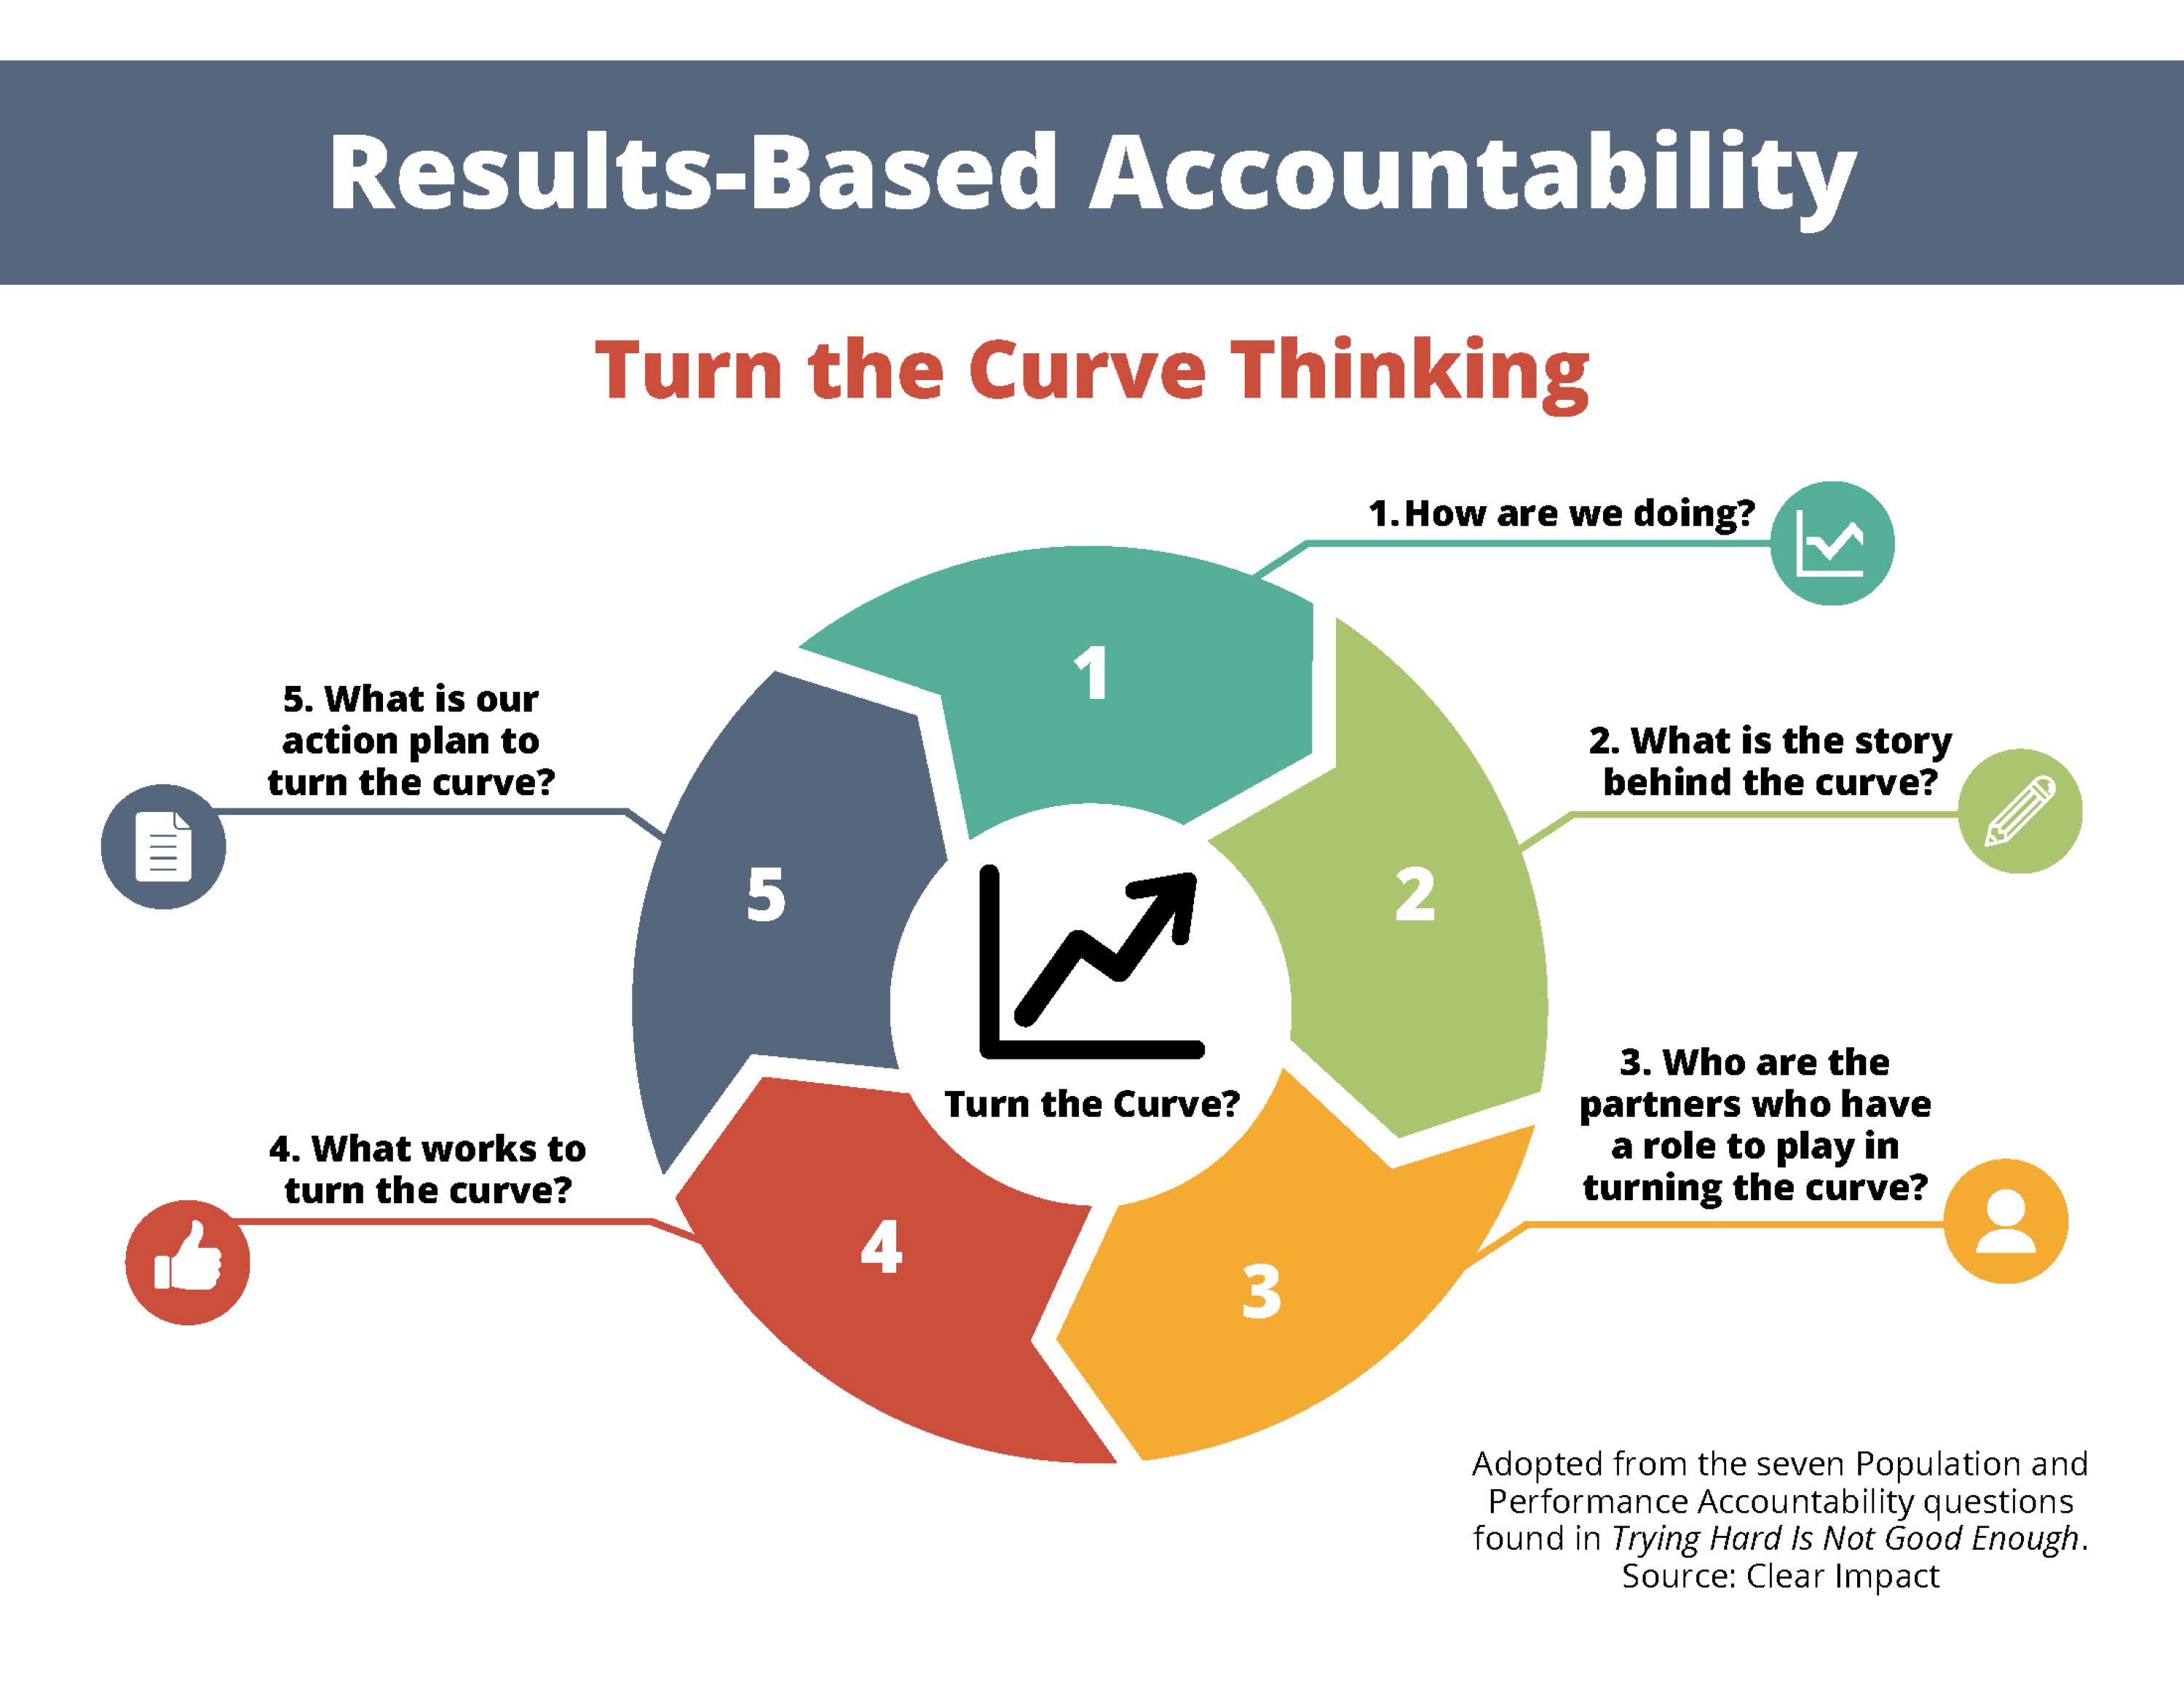
\includegraphics{pages/Attachments/Introduction/RBATurningtheCurve.png}

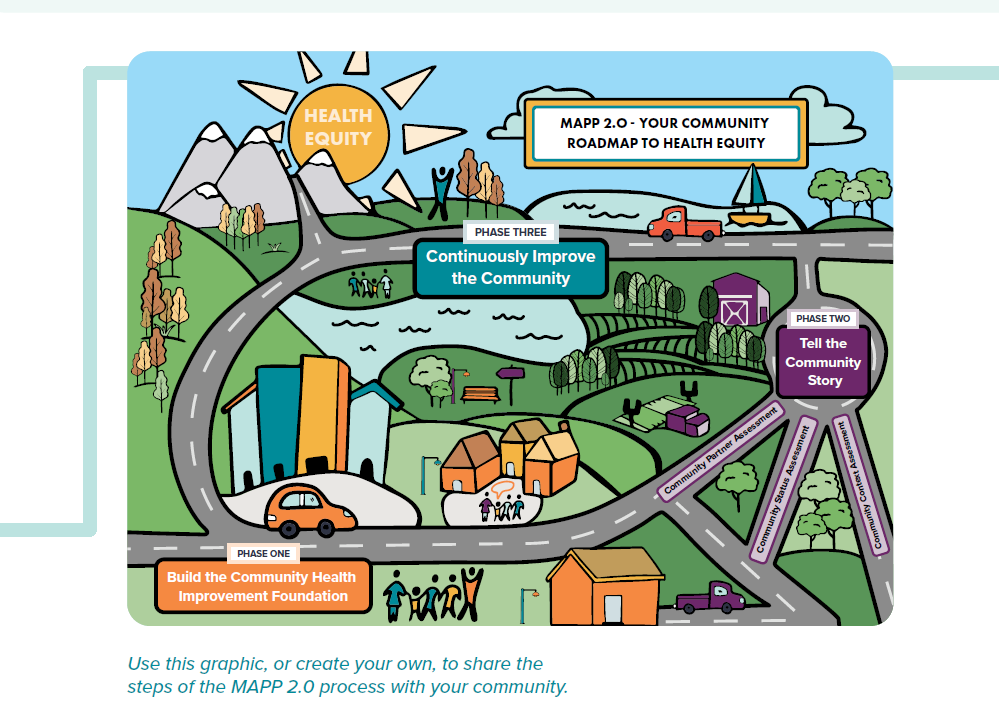
\includegraphics{pages/Attachments/Introduction/MAPP.png}

Thank you to the individuals, organization, and partners who have been
involved throughout the health assessment and planning process. A
special thank you to Patrick Olson, Data Analyst, for assisting PNM CHS
with gathering data from a variety of state and national sources in the
development of a more comprehensive Community Health Assessment to meet
public health accreditation standards and measures, Assessment and
Surveillance Foundational Public Health capability and inform meaningful
local action.

Thank you to the community members and partners of Polk, Norman and
Mahnomen Counties for participating in the community health surveys and
conversations.

We welcome your continued feedback and engagement. Comments or questions
regarding this report can be direct to: Sarah Reese,
Polk-Norman-Mahnomen CHS Administrator at 218-281-3385.

\bookmarksetup{startatroot}

\chapter{\texorpdfstring{\vspace{-2cm} Local
Input}{ Local Input}}\label{local-input}

\section{Polk-Norman-Mahnomen Community Health Survey
(2022)}\label{polk-norman-mahnomen-community-health-survey-2022}

Polk, Norman, and Mahnomen Community Health Services (CHS) conducted a
survey consisting of questions related to general, mental, oral health,
access to health care, impact of COVID-19 on health and quality of life,
substance use and community wellbeing. The survey was completed by 855
adult individuals. Out of the 855 survey responses, 821 were included in
the analysis as the remaining 34 respondents were not from the PNM
region.

Summary

\begin{itemize}
\item
  ``Poor'' health status was primarily reported by White and Black or
  African American population.
\item
  About 26\% of people experienced delay in seeking professional help
  for mental health during the pandemic and this was mainly because the
  mental health care was expensive, or they did not think that the
  problem was serious enough.
\item
  Most reported reason for delay in obtaining oral health care were
  expense, unable to get an appointment and lack of insurance coverage.
\item
  47\% of survey respondents consume alcohol, tobacco, or illegal drugs.
  Stress (16\%) and boredom (13\%) are the primary reason for the
  increase in substance use since March 2020.
\item
  Majority of respondents received health information from social media,
  family, friends, health officials or county media website and
  television news. However, about 37.63\% doubted whether the source was
  trustworthy. 19\% of people also had issue with understanding medical
  terms and about 12\% did not know where to find health information.
\item
  People with an annual income less than \$20,000 and between
  \$35,000-\$49,999 mainly reported worsening of financial situation.
\item
  About 8\% of survey respondents faced transportation issues and they
  reported to be from 25-44 years of age.
\end{itemize}

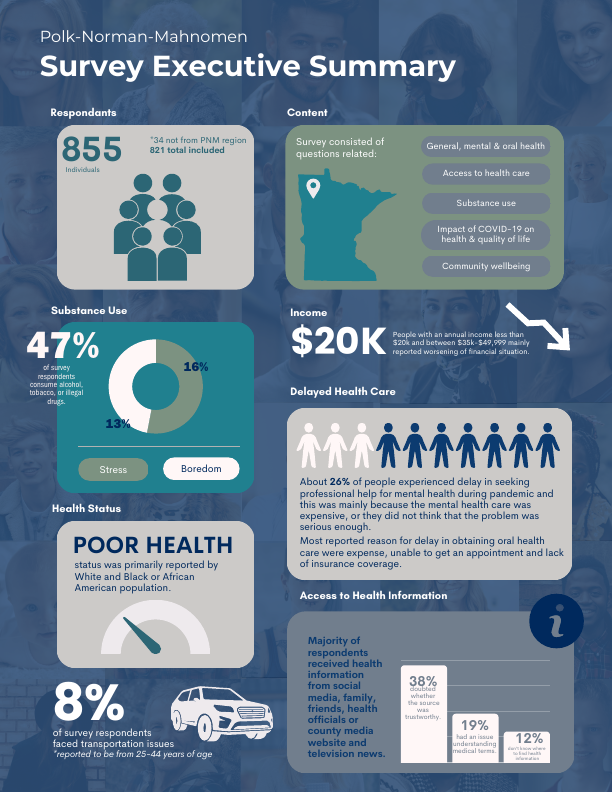
\includegraphics{pages/Attachments/localInput/surveyExeSummary.png}

\section{Polk-Norman-Mahnomen Environmental Scan
Survey}\label{polk-norman-mahnomen-environmental-scan-survey}

Polk, Norman, and Mahnomen Community Health Services (CHS) reached out
to 42 alcohol retailers in May and June of 2023 to learn more about how
our youth may be exposed to THC in our area.

\begin{itemize}
\item
  18/42 establishments were within 1000 feet of a school or
  park/playground.
\item
  36/42 advertised the sale of alcohol outside their establishment.
\item
  13/42 had exterior signage regarding minimum purchase age
\item
  35/42 had interior signage regarding purchase age.
\item
  5/42 had signage related to the health risks of drinking alcohol.
\item
  7/42 establishments were found to sell THC products (1 liquor store, 1
  vape shop, 5 bars/bar and grills)
\item
  4/7 sold edibles
\item
  3/7 sold THC-infused beverages
\item
  1/7 sold other THC products/paraphernalia.
\end{itemize}

\section{Polk County Opioid Funding Prioritization
Survey}\label{polk-county-opioid-funding-prioritization-survey}

The Polk County Opioid Funding Prioritization Survey gathered input from
community members to guide the allocation of over \$3 million from the
national opioid settlement. The survey, conducted from June 12 to July
24, 2023, received 137 responses, with a majority prioritizing
prevention, treatment, and recovery support. Key areas identified for
funding include primary prevention, community development, and treatment
expansion. The survey also highlighted the importance of harm reduction
strategies such as overdose reversal and social detox. The results have
shaped the county's approach to addressing the opioid crisis over the
next 18 years Polk County (2023).

For more information please use the following url
https://www.co.polk.mn.us/DocumentCenter/View/2073/Polk-County-Opioid-Funding-Prioritization-Survey-Results?bidId=

Link to site Opioid Settlement Advisory Council
https://www.co.polk.mn.us/546/Opioid-Settlement-Advisory-Council

\section{Community Heath Needs Assessment \& Community Needs Assessments
Partner
Inventory}\label{community-heath-needs-assessment-community-needs-assessments-partner-inventory}

This is an accumulation of most recent Community Health Needs
Assessments (healthcare partners) and Community Needs Assessments
(Community Action agencies) of our partners. It is not intended to be
all encompassing; partners continue to have current and emerging
priorities in response to the needs of community.

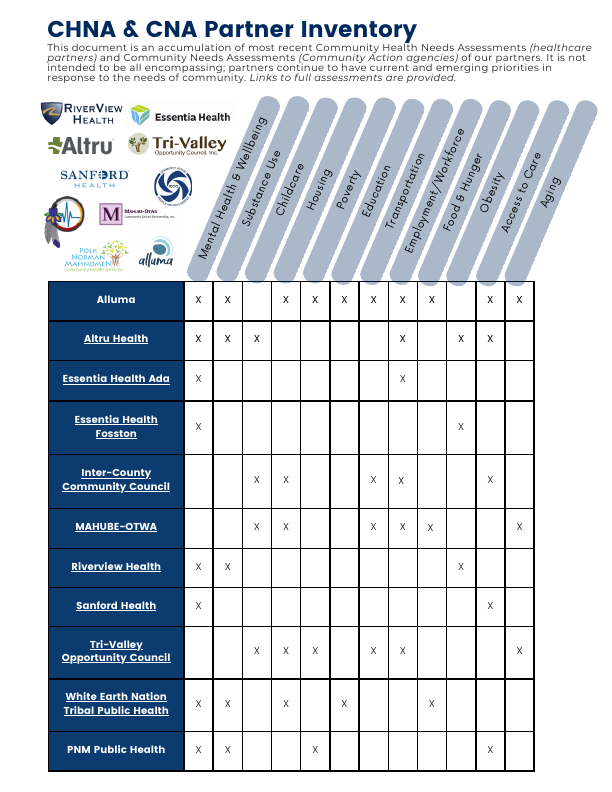
\includegraphics{pages/Attachments/localInput/cHNACNAPartnerInventory.png}

\bookmarksetup{startatroot}

\chapter{Physical Health}\label{physical-health}

Certain environments can contain factors that impact our health. We may
be unaware of the potential risks in our homes, workplaces, schools, or
other areas in our communities, which could increase our chances of
developing medical conditions. Lack of awareness can be detrimental to
our health. The following environmental indicators are not meant to
alarm but to educate us about the environmental factors we may encounter
in our communities, helping us become more informed and proactive.

\subsection{Tickborne Disease Risk}\label{tickborne-disease-risk}

As shown on the following map, Polk, Norman, and Mahnomen are identified
as high-risk areas for tickborne diseases, including Lyme disease.
During tick season, we should be proactive in preventative measures,
such as using tick repellents and performing regular tick checks, to
reduce the risk of infection. Our high-risk area underscores the
importance of awareness to be proactive in our health practices. By
staying informed and vigilant, we can better protect ourselves and our
communities. Remember, early detection and prompt removal of ticks can
lower the chances of disease transmission.

\begin{figure}[H]

\centering{

\href{https://www.health.state.mn.us/diseases/lyme/highrisk.html}{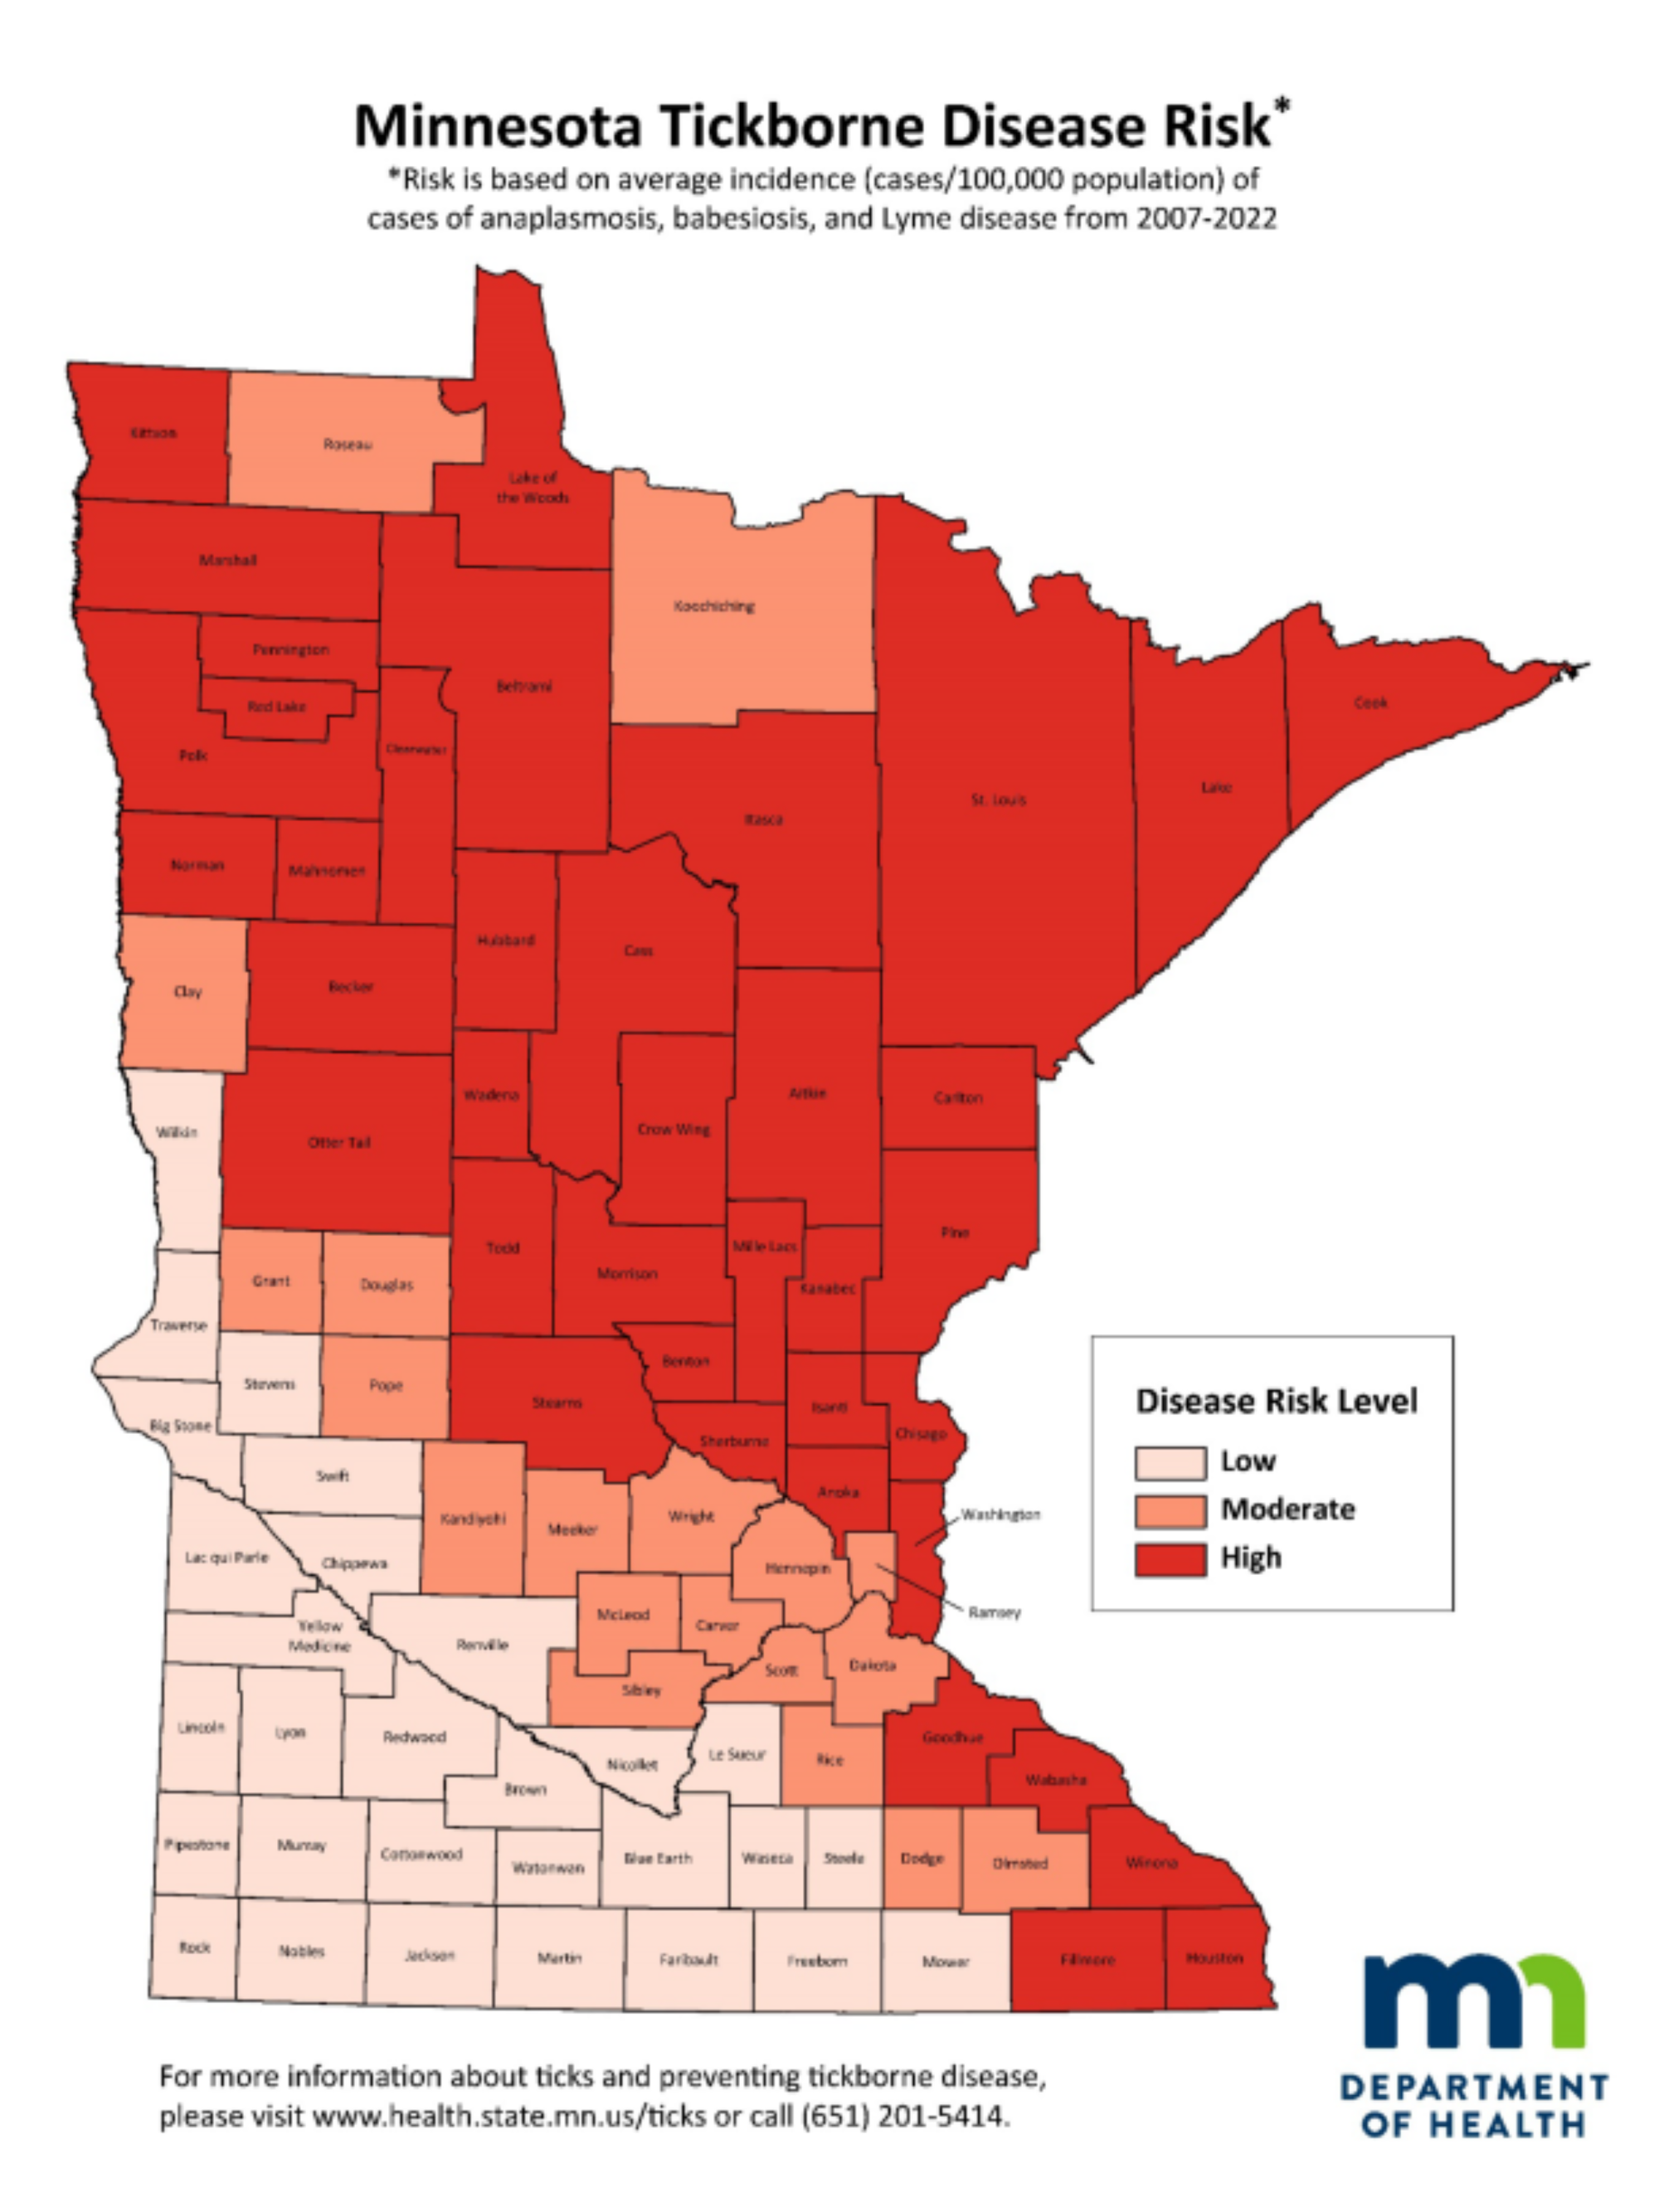
\includegraphics{pages/Attachments/popEnvironmentalHealth/mnMap_countyTickBorneRisk.png}}

}

\caption{\label{fig-tickborneRisk}For more resources, please click
anywhere on the map}

\end{figure}%

\subsection{Arsenic}\label{arsenic}

Arsenic can be found in drinking water. Testing is vital in learning if
your water has arsenic. The MDH recommendation is to test a private well
at least once for arsenic. Chronic arsenic exposure has shown to be a
risk factor for some cancers and also can impact a child's development .

From 2008 to 2021, 58.9\% (399 out of 465) of wells tested in Polk
County had arsenic levels greater than 2 µg/L, and 20.8\% (141 out of
465) exceeded 10 µg/L. Norman County had higher percentages, with 73.6\%
(131 out of 178) of wells testing above 2 µg/L and 42.7\% (76 out of
178) exceeding 10 µg/L. Mahnomen County showed similar results to Norman
County, with 77.5\% of wells testing above 2 µg/L and 41.9\% exceeding
10 µg/L, based on a total of 267 tests Minnesota Department of Health
(2008-2021).

\begin{figure}[H]

\centering{

\href{https://mndatamaps.web.health.state.mn.us/interactive/wells.html}{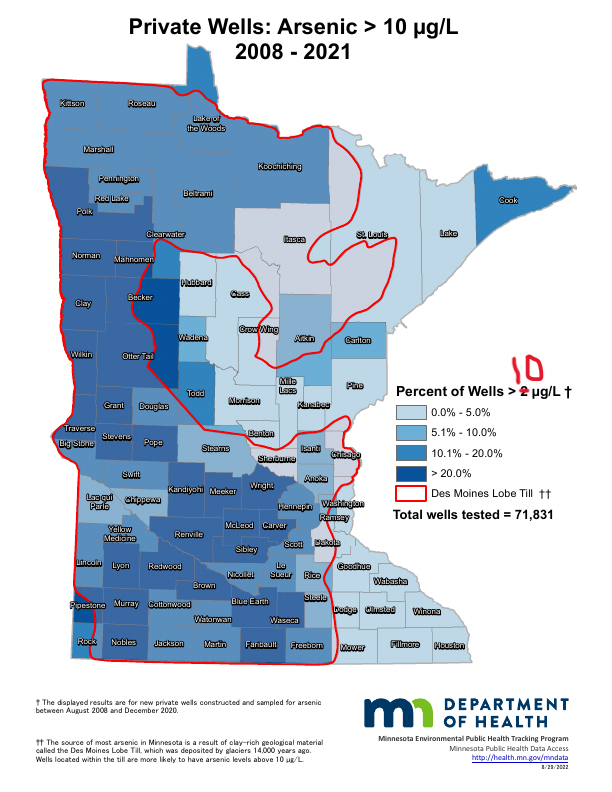
\includegraphics{pages/Attachments/popEnvironmentalHealth/mnMap_countyAs10ugLDML.png}}

}

\caption{\label{fig-privateWellsAs}For more resources, please click
anywhere on any of the maps}

\end{figure}%

\subsection{Radon}\label{radon}

From 2010 to 2020 Minnesota Department of Health (2024), Minnesota
averaged 93.5 radon tests per 10,000 properties each year. In
comparison, Mahnomen had 28.8 tests, Norman had 50.4, and Polk had 38.7
tests per 10,000 properties annually.

Regarding radon levels, 40.3\% of properties tested in Minnesota had
radon levels of 4 pCi/L or higher. In Polk, 70\% of properties tested
had high radon levels, while Norman had 56.6\%, and Mahnomen had 57.7\%.

\begin{figure}[H]

\centering{

\href{https://mndatamaps.web.health.state.mn.us/interactive/radon.html}{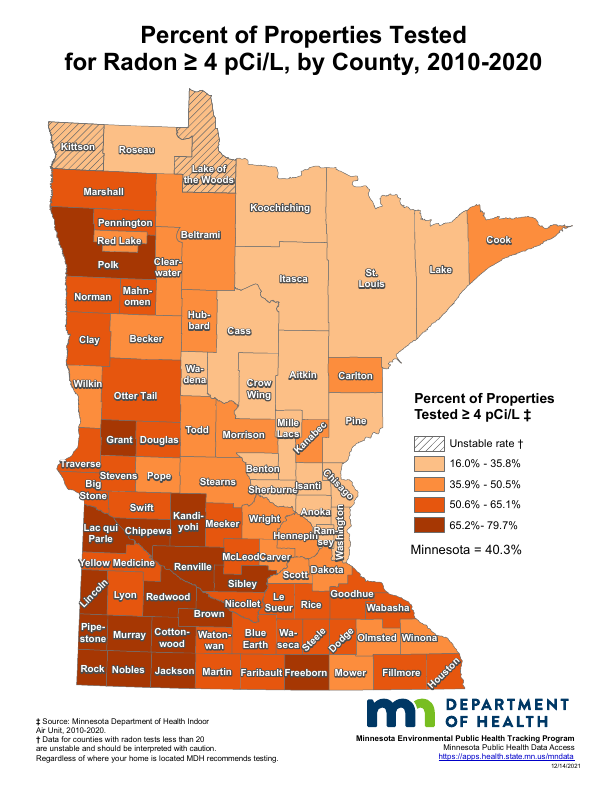
\includegraphics{pages/Attachments/popEnvironmentalHealth/mnMap_countyRn4pCiL.png}}

}

\caption{\label{fig-radon}For more resources, please click anywhere on
any of the maps}

\end{figure}%

\subsection{Toward Zero Deaths Fatal/Serious Injury
Crashes}\label{toward-zero-deaths-fatalserious-injury-crashes}

It is important to know any potential high crash areas in our counties.
It is very encouraging that we don't see any red, purple, or blue on the
maps developed by Toward Zero Deaths (2023). It is even for a five-year
time period, and we still don't see alarming signs of concern resulting
in serious injury or death. This may reflect the effectiveness of our
local road safety measures and community awareness. Continuing to
prioritize safe driving practices will help maintain and improve these
outcomes.

\begin{figure}[H]

\begin{minipage}{0.33\linewidth}
\href{https://www.minnesotatzd.org/regions/westcentral}{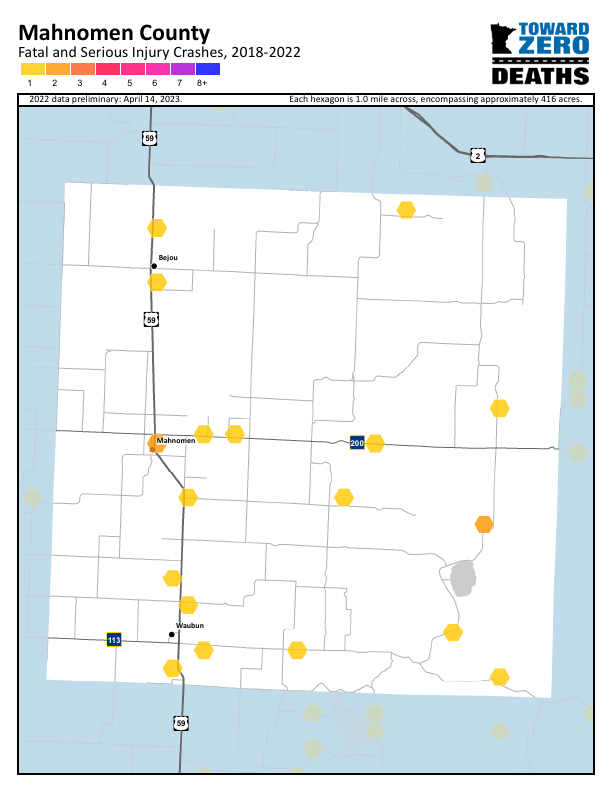
\includegraphics{pages/Attachments/popEnvironmentalHealth/countyMahnomenMap_crashes2019_2023.png}}\end{minipage}%
%
\begin{minipage}{0.33\linewidth}
\href{https://www.minnesotatzd.org/regions/northwest}{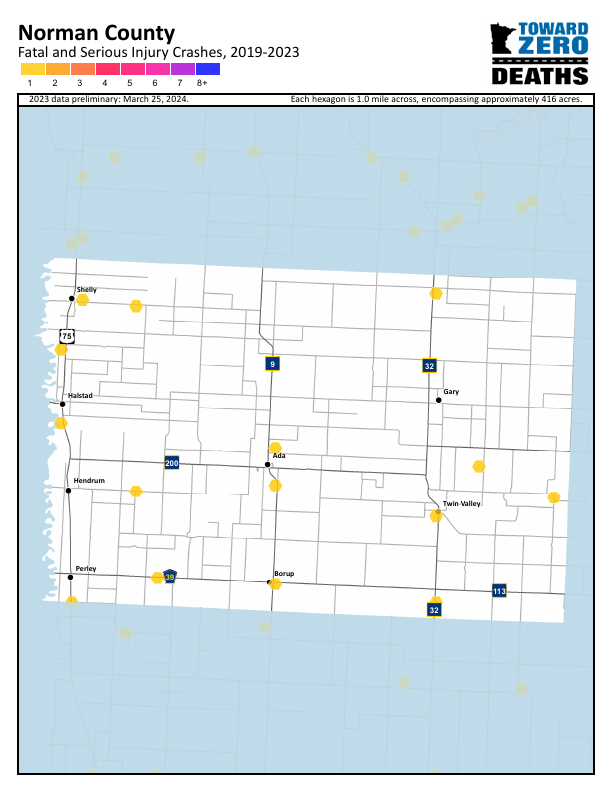
\includegraphics{pages/Attachments/popEnvironmentalHealth/countyNormanMap_crashes2019_2023.png}}\end{minipage}%
%
\begin{minipage}{0.33\linewidth}
\href{https://www.minnesotatzd.org/regions/northwest}{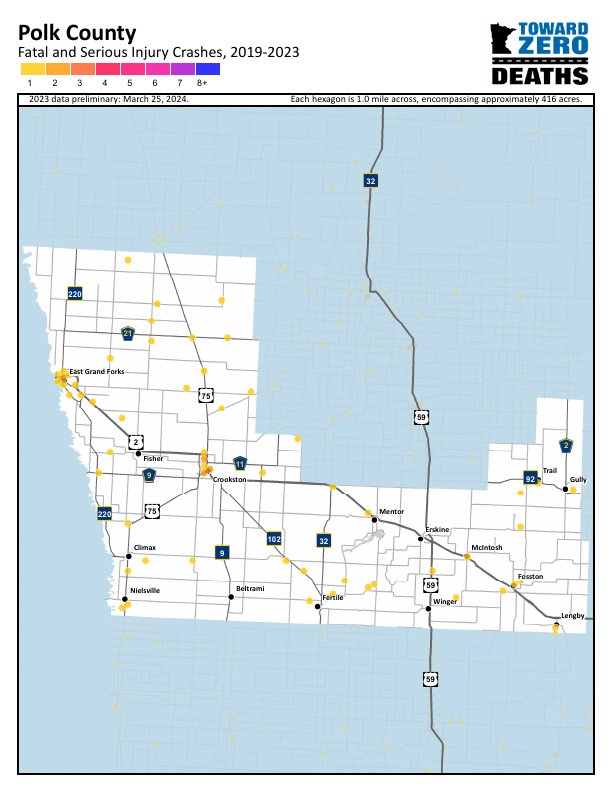
\includegraphics{pages/Attachments/popEnvironmentalHealth/countypolkMap_crashes2019_2023.png}}\end{minipage}%

\caption{\label{fig-seriousCrash}For more resources, please click
anywhere on any of the maps}

\end{figure}%

\phantomsection\label{refs}
\begin{CSLReferences}{1}{0}
\bibitem[\citeproctext]{ref-arsenic2008_2021}
Minnesota Department of Health. 2008-2021. {``Private Wells - Arsenic
(2008-2021).''}
\url{https://mndatamaps.web.health.state.mn.us/interactive/wells.html}.

\bibitem[\citeproctext]{ref-mnhealthRadon}
---------. 2024. {``Radon.''}
\url{https://data.web.health.state.mn.us/radon}.

\bibitem[\citeproctext]{ref-polkOpioid}
Polk County. 2023. {``Polk County Opioid Funding Prioritization.''}
\url{https://www.co.polk.mn.us/DocumentCenter/View/2073/Polk-County-Opioid-Funding-Prioritization-Survey-Results?bidId=}.

\bibitem[\citeproctext]{ref-crashSite2023}
Toward Zero Deaths. 2023. {``TZD Regions.''}
\url{https://www.minnesotatzd.org/regions}.

\end{CSLReferences}




\end{document}
